\subsection{\acl{BDD}}
\label{subsec:bdd}
\acf{BDD} is a software development practice intricately woven into the framework of agile methodologies, which signifies a profound transformation in conventional software engineering approaches. Position itself as a dynamic response to prevalent challenges by prioritizing user behavior and aligning closely with business needs. Based on the integration of concepts from both \ac{TDD} and \ac{DDD}, \ac{BDD} transcends traditional development paradigms.

\ac{BDD} stands out as a departure from the typical \ac{TDD} methodology, where the primary focus is on writing tests for isolated code units, with a predominant technical viewpoint. Instead, \ac{BDD} broadens its perspective, bridging the gap between technical and business aspects. It achieves this by incorporating viewpoints from both spheres, redirecting the evaluation from individual code segments to the holistic assessment of the application's behavior from the user's standpoint. This strategic change not only enhances communication, but also fosters collaboration between developers, testers, and business stakeholders, as evidenced by previous research~\cite{smart2023bdd,pereira2018behavior}.

In response to the challenges posed by the highly technical and code-centric nature of \ac{TDD}, \ac{BDD} introduces an innovative testing methodology. Rooted in a user-centric philosophy, test cases are structured using a language that mirrors natural language. This linguistic clarity serves as a catalyst for effective collaboration, ensuring a shared understanding among team members throughout the software development lifecycle.

\subsection{Gherkin}
\label{subsec:gherkin}

Gherkin is a \ac{DSL} prominently utilized in the domain of \ac{BDD}. It is used to create requirements and tests in a clear and human-readable format. Gherkin's syntax follows a systematic Given-When-Then structure, interweaving natural language expressions, as demonstrated in \cref{lst:withdrawcash}. Therefore, we focus on the end-user's perspective and business requirements rather than the underlying technical implementation.

\begin{listing}[!ht]
\caption{Exemplary feature file with one scenario}
\label{lst:withdrawcash}
\inputminted{gherkin}{files/code/atm.feature}
\end{listing}

 Gherkin employs a distinct set of keywords to delineate various aspects of test scenarios. Notably, it utilizes the \textit{Feature} keyword to expound upon the primary functionality of the feature under examination, \textit{Scenario} for specifying individual use cases within the feature, \textit{Given}-steps to establish initial context or preconditions, \textit{When}-steps for denoting the event or action triggering the scenario, and \textit{Then}-steps for articulating anticipated outcomes for validation\footnote{It is imperative to acknowledge that this chapter does not exhaustively cover all Gherkin keywords, but rather focuses on those pertinent to our study. A comprehensive list is available at \href{https://cucumber.io/docs/gherkin/reference/\#keywords}{https://cucumber.io/docs/gherkin/reference}}. Furthermore, the \textit{And} keyword facilitates the chaining of multiple steps of the same type, ensuring a logically granular and encapsulated representation of test steps. This structural arrangement cultivates a shared understanding among stakeholders about the expected behavior of the system, thereby mitigating the previously delineated structural challenges. In particular, this structure harmonizes well with user stories and other agile methodologies, providing sufficient structure for interpretation by frameworks such as Cucumber to map individual test steps to executable code (cf.~\cref{subsec:cucumber}).


\subsection{Cucumber}
\label{subsec:cucumber}
Cucumber, an open source software library, excels as a powerful tool to carry out \ac{BDD} tests. Functioning as a versatile framework, Cucumber facilitates the expression, automation, and validation of software requirements in a human-readable format. Its key role lies in promoting collaboration between non-technical stakeholders and developers, serving as a reliable bridge to ensure a shared understanding of project requirements. As a library designed explicitly for BDD testing, Cucumber enables the execution of automated tests based on Gherkin, effectively linking natural language descriptions with concrete test implementation steps.

\begin{figure}
    \centering
    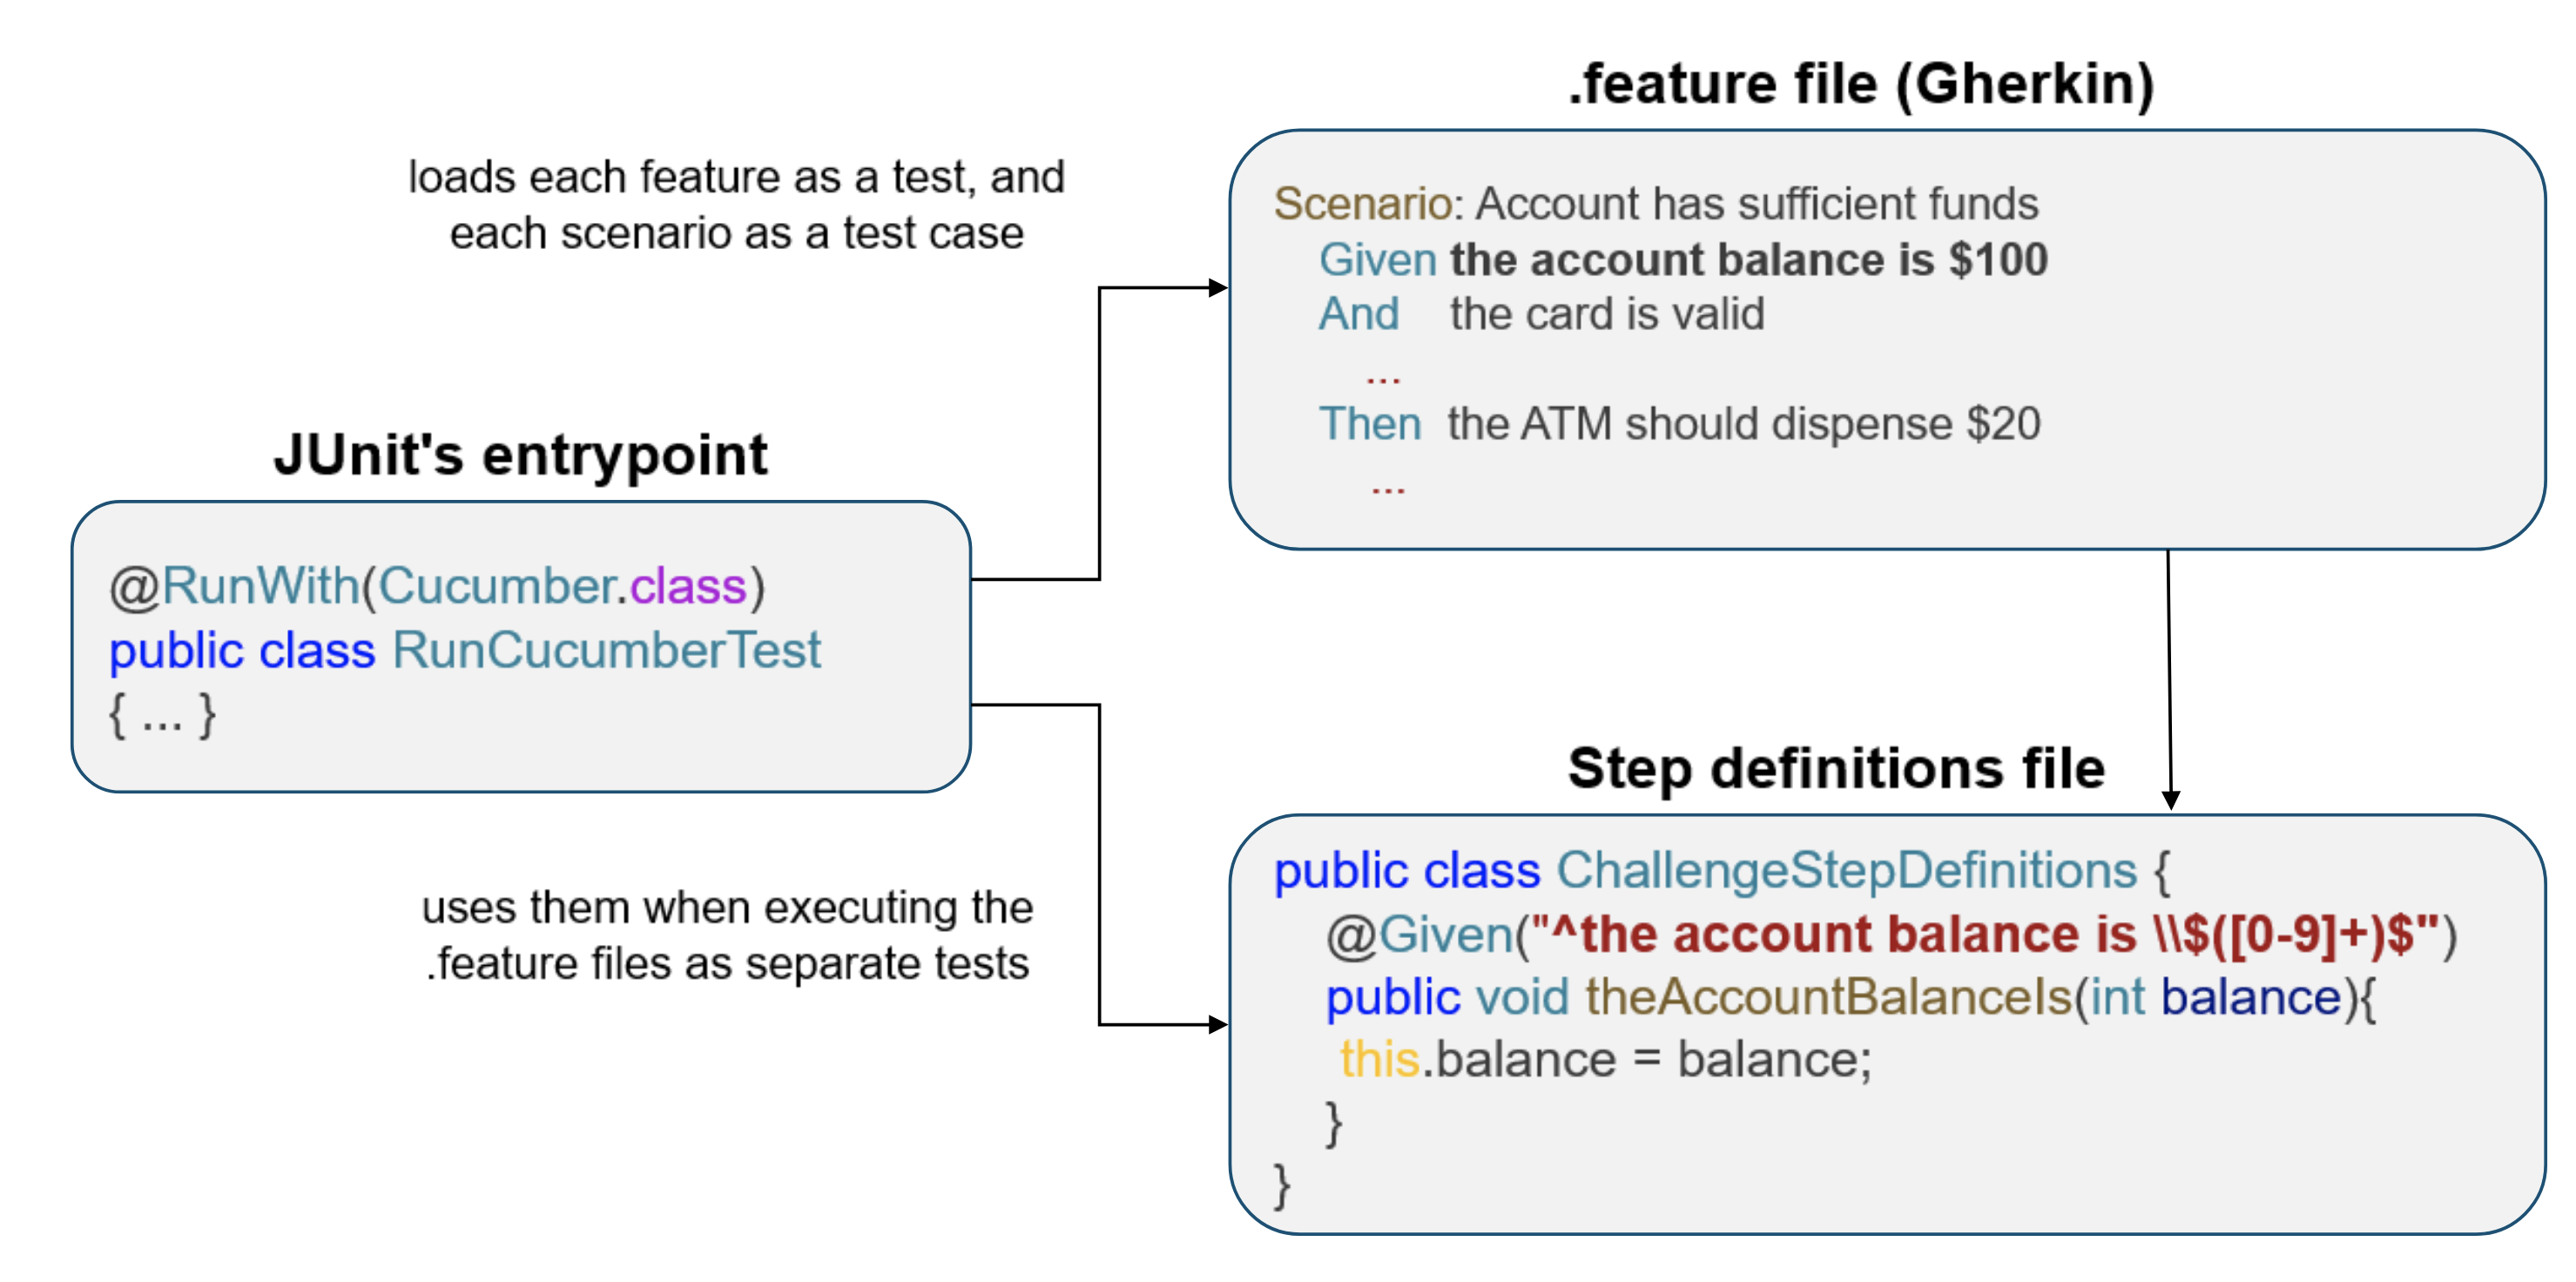
\includegraphics[width=\linewidth]{files/figures/cucumber_test_step_mapping.png}
    \caption{Illustration how Cucumber is used to link natural language clauses and their respective Java implimentations}
    \label{fig:cucumber-mapping}
\end{figure}

Based on the scenario in~\cref{lst:withdrawcash}, the corresponding ~\cref{fig:cucumber-mapping} illustrates the connection between the specified natural language test steps and their concrete code representations. This link relies on pattern matching through regular expressions. For example, the \textit{theAccountBalanceIs} function, annotated with \textit{@Given} and including a \ac{Regex}, aligns its execution with the type of test step and the defined \ac{Regex} pattern. By assigning values to instance variables, Cucumber maintains a shared context across test steps, ensuring a consistent and seamless testing flow.

\subsection{Distributed Systems}
\label{subsec:dissys}
A distributed system is a network of independent computers, running on multiple servers or nodes, that interact and synchronize their activities through the exchange of messages \cite{tanenbaum2007distributed}. These systems consist of components that collaboratively work towards a shared objective, presenting advantages in terms of performance, scalability, and redundancy when compared to centralized systems. The shift towards distributed systems is motivated by the inadequacies of non-distributed, centralized computing models, typified by a single monolithic server. Such centralized models have proven insufficient in addressing the increasing computational requirements and the need for enhanced system capabilities that could not be mitigated by vertically scaling a single system.

The distinctive feature of distributed systems lies in their avoidance of shared computing and memory resources, introducing complexities related to heterogeneity, scalability, and failure handling, among other challenges~\cite{coulouris2005distributed}. Non-distributed systems may struggle to effectively manage these challenges, leading to limitations in performance, scalability, and fault tolerance. Distributed systems, by distributing computational tasks across a network of interconnected computers, address these shortcomings.

For instance, consider a scenario where a centralized system, operating on a single powerful server, reaches the maximum capacity of available hardware resources. Upgrading the hardware of that single machine (vertically scaling), may become impractical or cost-prohibitive. In such situations, distributed systems offer a viable solution. By distributing the workload across multiple interconnected nodes, these systems enable parallel processing, allowing for efficient utilization of available resources beyond the constraints of a single machine. 

\subsection{\acl{RCE}}
\label{subsec:rce}

\ac{RCE} is an open-source application primarily developed at the \ac{DLR}. It is designed to facilitate the multidisciplinary engineering process, especially in complex system engineering such as aerospace, allowing users to integrate various disciplinary tools, define their dependencies and execute multidisciplinary workflows\cite{BODEN2021100759}. A key feature of \ac{RCE} is its ability to connect different \ac{RCE} instances in a distributed system, which greatly facilitates collaboration between various departments and specializations. This interconnected approach allows engineers from multiple disciplines to contribute their individual tools to a unified workflow, enhancing efficiency and reducing the propensity for errors in complex engineering projects. In this paper, our focus will be limited to those aspects of \ac{RCE} that are relevant to our project. Consequently, many features and advantages of \ac{RCE} that extend beyond the scope of our work will not be addressed herein. For a comprehensive presentation of \ac{RCE} as well as its capacity to facilitate multidisciplinary collaboration, the reader is directed to consult the detailed tool papers provided in \cite{BODEN2021100759,boden2019distributed}, which offer extensive insight into the broader applications and benefits of \ac{RCE}.